\documentclass[11pt]{article}

% colors
\usepackage[table]{xcolor}
\definecolor{maroon}{RGB}{153,0,18}
\definecolor{lime}{RGB}{190,213,88}
\definecolor{sand}{RGB}{217,202,179}
\definecolor{fire}{RGB}{144,50,61}
\definecolor{brick}{RGB}{94,11,21}
\definecolor{olive}{RGB}{117,109,84}
\definecolor{lavpink}{RGB}{172,123,132}
\definecolor{darkpurp}{RGB}{49,10,49}
\definecolor{salmon}{RGB}{204,90,113}
\definecolor{mauve}{RGB}{94,73,85}
\definecolor{greyblue}{RGB}{125,132,145}
\definecolor{greypurp}{RGB}{68,56,80}
\definecolor{brightpurp}{RGB}{96,20,255}

% packages (please add in alphabetical order)
\usepackage{adjustbox}
\usepackage{amsfonts}
\usepackage{amsmath}
\usepackage{amssymb}
\usepackage{array}
\usepackage{bm}
\usepackage{booktabs}
\usepackage{caption}
\usepackage{epstopdf}
\usepackage{float}
\usepackage[margin=1in]{geometry}
\usepackage{graphicx}
\usepackage[colorlinks=true, linkcolor=brightpurp, citecolor=brightpurp, urlcolor=salmon]{hyperref}
\usepackage{lipsum}
\usepackage{longtable}
\usepackage{mathtools}
\usepackage{multirow}
\usepackage{natbib}
\usepackage{rotating}
\usepackage{setspace}
\usepackage{subcaption}
%\usepackage{threeparttable}
\usepackage{threeparttablex}
\usepackage{xr}
\usepackage[printwatermark]{xwatermark}


\newcolumntype{L}[1]{>{\raggedright\let\newline\\\arraybackslash\hspace{0pt}}m{#1}}
\newcolumntype{C}[1]{>{\centering\let\newline\\\arraybackslash\hspace{0pt}}m{#1}}
\newcolumntype{R}[1]{>{\raggedleft\let\newline\\\arraybackslash\hspace{0pt}}m{#1}}

% commands
\newcommand{\mr}{\multirow}
\newcommand{\mc}{\multicolumn}


\begin{document}

\section{Labor Income Profiles, ABC/CARE}

\begin{center}
\begin{figure}[H] 
\caption{Forecasted Labor Income Profile, Males}
\label{figure:youlabel}
\centering
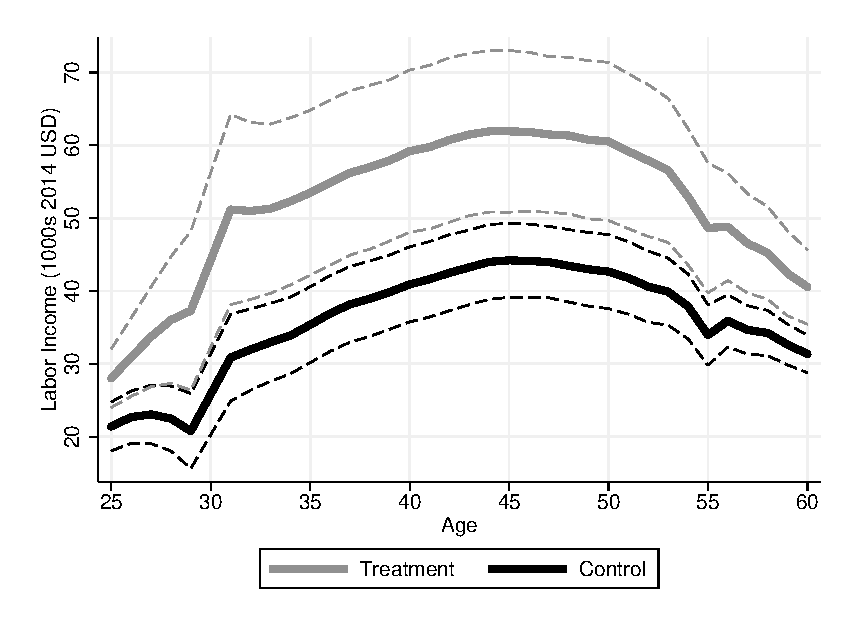
\includegraphics[width=.55\columnwidth]{output/labor_25-60_male.eps}
\floatfoot{
\footnotesize
Note: This plot displays the labor income profiles for ABC/CARE males by treatment status, based on forecasts that combine data from the Panel Study of Income Dynamics (PSID) and the Children of the National Longitudinal Survey of Youth 1979 (cNLSY79).
}
\end{figure}
\end{center}

\begin{center}
\begin{figure}[H] 
\caption{Forecasted Labor Income Profile, Females}
\label{figure:youlabel}
\centering
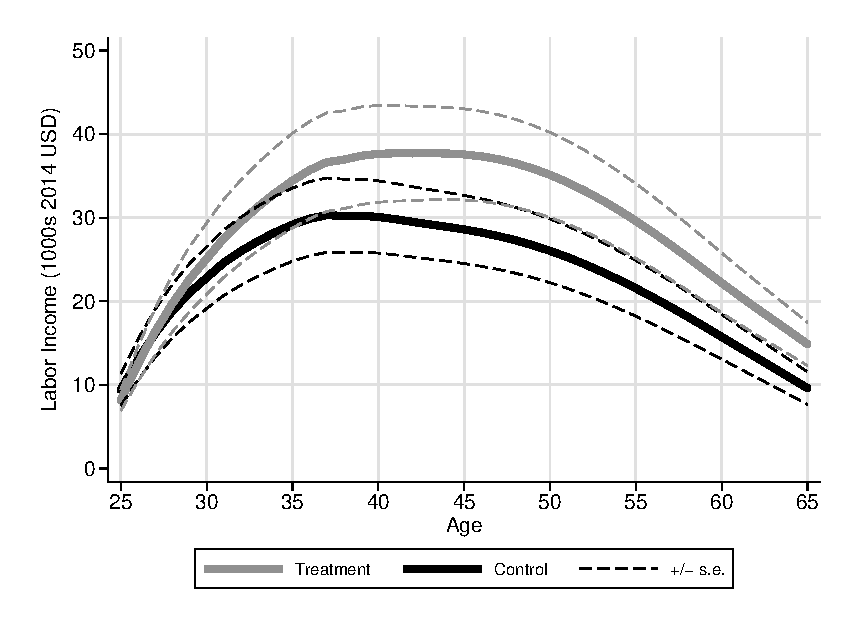
\includegraphics[width=.55\columnwidth]{output/labor_25-60_female.eps}
\floatfoot{
\footnotesize
Note: This plot displays the labor income profiles for ABC/CARE females by treatment status, based on forecasts that combine data from the Panel Study of Income Dynamics (PSID) and the Children of the National Longitudinal Survey of Youth 1979 (cNLSY79).
}
\end{figure}
\end{center}


\end{document}